\section{Lists}
%\textit{Child and Configuration lists and their adapters\\
%Lister generelt, hvad er Android filosofien bag lister}
Android provide a built-in \texttt{ListView}, which can be modified to match any list, that the developer wish to create, as shown in \autoref{fig:listview_example}.

\begin{figure}[H]
	\centering
		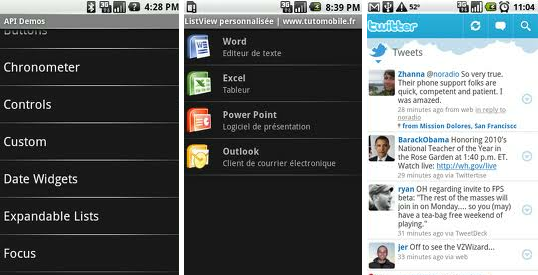
\includegraphics[width=\textwidth]{Images/Implementation/listview_example.png}
	\caption{Three examples of how \texttt{ListView} can be modified.}
	\label{fig:listview_example}
\end{figure}

\subsection{Benefits and Limitations}
%\textit{ Hvad er fordelen ved at bruge lister frem for at lave sin egen liste af textviews\\
%ADAPTERS\\
%Hvor langt tilbage er lister understøttet\\}
The advantage of a \texttt{ListView} is, that it can be modified to whatever the developer want it to look like.
This is done by making an adapter with the changes the developer want to make to the design. An example of how to use this adapter can be seen in \autoref{code:listview_adapter_example}.

\begin{figure}[H]
	\centering
	\begin{lstlisting}
View v = list_item_view;
	if (v == null) {
		LayoutInflater li = (LayoutInflater) getContext().getSystemService(
				Context.LAYOUT_INFLATER_SERVICE);
		v = li.inflate(R.layout.profile_list, null);
	}
	Child c = items.get(position);
	if (c != null) {
		ImageView iv = (ImageView) v.findViewById(R.id.profilePic);
		TextView tv = (TextView) v.findViewById(R.id.profileName);

		if (iv != null) {
			iv.setImageResource(R.drawable.default_profile);
		}
		if (tv != null) {
			if (c.name == "Last Used") {
				tv.setText(R.string.last_used);
			} else if (c.name == "Predefined Profiles") {
				tv.setText(R.string.predefined);
			} else {
				tv.setText(c.name);
			}
		}
	}
\end{lstlisting}
	\caption{The WOMBAT implementation of a \texttt{ListView} \texttt{ArrayAdapter} modified to use a list of profiles.}
	\label{code:listview_adapter_example}
\end{figure}

The \texttt{ListView} have an interface, \texttt{OnItemClickListener}, which works like any other clickable item in Android.

\subsection{Lists in WOMBAT}
%\textit{ Hvordan bruger vi lister\\
%Child listen, SubProfile listen\\
%Hvordan har det indflydelse på applikationen\\}
Figure \ref{code:listview_adapter_example} is the actual implementation of the child list in WOMBAT. The difference from the \textttArrayAdapter} used in the profile list and the configuration list, is that the configurations is designed to use a text field with a description of the timer.
The configurations list only requires another layout to be constructed, this layout contains the extra \texttt{TextView}.\\

The \texttt{OnItemClickListener} of the child fragment ensures that the configuration fragment and customi object, described in \autoref{sec:backend}, is updated. \autoref{code:listview_onclick_example} is an example of the child fragment \texttt{ListView}.

\begin{figure}[H]%
		\begin{lstlisting}
			public void onListItemClick(ListView lv, View view, int position, long id) {
				// Update the fragments
				SubProfileFragment detf = (SubProfileFragment) getFragmentManager()
						.findFragmentById(R.id.subprofileFragment);
				CustomizeFragment custF = (CustomizeFragment)getFragmentManager().findFragmentById(R.id.customizeFragment);
				custF.setDefaultProfile();
				
				if (detf != null) {
					// Marks the selected profile in the guard singleton
					guard.profilePosition = position; 
					guard.publishList().get(position).select();
					guard.profileID = guard.publishList().get(position).getProfileId();
					detf.loadSubProfiles();
				}
			}
		\end{lstlisting}
	\caption{Example of the \texttt{OnClickListener} of the child fragment.}
	\label{code:listview_onclick_example}%
\end{figure}

